\subsection{データの抽象化入門}
プロシージャーを作ることによって, 複合の操作だけでなく,
抽象化として見ることができる.

複合のデータについても同じことができ, それをデータの抽象化という.
プログラムにおいて, 抽象的にデータを扱うというのは,
可能な限りデータはどう表現されているか関係なく扱うことである.
それに対して, 具体的なデータはプログラムと関係なく定義されているものである.

具体的なデータと抽象的なデータの間に変換するために, セレクターとコンストラクタを用いる.
%
\subsubsection{有理数での算術}
有理数を使って四則演算を実装したいとする. 分数を表す方法がある前提で考えて,
分子と分母から分数を返す\lstinline{make-rat}, 分数から分子を返す\lstinline{numer},
分数から分母を返す\lstinline{denom}という3つのプロシージャが存在するとする.

分数の四則演算は

\begin{align*}
  &\frac{n_1}{d_1} + \frac{n_2}{d_2}  = \frac{n_1d_2 + n_2d_1}{d_1d_2}
  & \frac{n_1}{d_1}\cdot \frac{n_2}{d_2} = \frac{n_1n_2}{d_1d_2}\\
  &\frac{n_1}{d_1} - \frac{n_2}{d_2} = \frac{n_1d_2 - n_2d_1}{d_1d_2}
  & \frac{n_1/d_2}{n_2/d_2} = \frac{n_1d_2}{d_1n_2}\\
  &\frac{n_1}{d_1} = \frac{n_2}{d_2} \Leftrightarrow n_1d_2 = n_2d_1
\end{align*}
\noindent
のように定義できるので, 以上の3つのプロシージャがあれば, 問題なくそれぞれの
演算を問題なく実装できる. 例えば, 足し算は以下のように実装できる.

\begin{lstlisting}[basicstyle=\footnotesize,title=分数の足し算]
(define (add-rat x y)
  (make-rat (+ (* (numer x) (denom y))
               (* (numer y) (denom x)))
            (* (denom x) (denom y))))
\end{lstlisting}
\vspace{5mm}

Lispにはペアというデータ構造が存在しており, 2つのデータを1つの構造として表現できる.
\lstinline{cons}で2つの要素から1つのペアを作ることができ, \lstinline{car}で
1つ目の要素を取り出し, \lstinline{cdr}で2つ目の要素を取り出す.
ペアを用いると, 分数を自然に表現することができる.

\begin{lstlisting}[basicstyle=\footnotesize,title=分数の表現]
(define (make-rat n d) (cons n d))
(define (numer x) (car x))
(define (denom x) (cdr x))
\end{lstlisting}

%
\subsubsection{抽象化の壁}
データを扱う時に複数の抽象化のレイヤについて考えられる.
分数の例で考えると, 以下の図のようなレイヤが考えられる.

\begin{figure}[h]
  \centering
  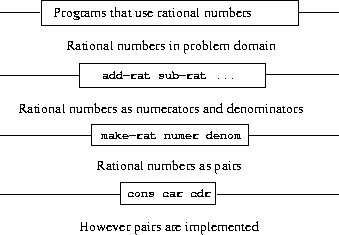
\includegraphics[width=12cm,height=5cm]{imgs/abstraction-barrier.png}
\end{figure}

ここで抽象化のレベルが4つで分かれている. 最も上のレイヤは分数を扱うプログラムが使うもので,
実際分数はどう表現されているかも, どう四則演算が定義されているのかが分からなくても四則演算が
できるレベルである. その下のレイヤでは, 実際四則演算の実装である. そこで分数のセレクタと
コンストラクタを用いるが, その実装に依存しない. その下のレイヤはセレクタとコンストラクタの実装で,
ペアを用いるが今回もその実装に依存しない. 最も下のレイヤはペアの実装である.

そのレイヤ分けの主な利点はプログラムの保守性と柔軟性の向上である.
下のレイヤの実装に依存しないので, データをどう表現するかが変わらない限り,
実装が変わっても影響が受けない.

